\chapter{The UK Bombe}

\section{Motivating Example}

\section{Changes to Enigma}

Starting in 1940, the German's enhanced the security of their 
key distribution. As discussed in CITE the \emph{Grundstellung} rotor 
position was sent along with the daily key and an operator chose a \emph{Spruchschlusse} to 
encode twice at the start of a message. Later iterations of this protocol removed the \emph{Grundstellung}
from key sheets.
\\\\These new key sheets contained the following columns
columns \emph{Tag/Datum}, \emph{Walzenlage}, \emph{Ringstellung}, \emph{Steckerverbindungen}, and \emph{Kenngruppen} 
\\\\Notice the removal of the \emph{Grundstellung} as well as the addition of the \emph{Kenngruppen}. The \emph{Kenngruppen} were a set of 
four trigrams used to identify which setting was being used to encode a message, this is particularly useful if trying to decode a message using a prior day's key. 
The operator would choose a trigram from the the \emph{Kenngruppen}, append two letters to the front of the trigram,
and this five letter combination (known as the \emph{Buchstabenkenngruppe}) would preceed the message being sent. If a message
was sent in multiple segments, multiple \emph{Buchstabenkenngruppe} were used to start each segment.
\\\\When sending a message the operator was to use the following protocol
\begin{enumerate}[I.]
\item The time at which the message was sent is listed
\item The number of parts which the message contained is listed
\item Which message part is being sent is listed
\item The length of the message part (not including \emph{Buchstabenkenngruppe}) is listed
\item A \emph{Grundstellung} rotor position is chosen and listed 
\item A \emph{Spruchschlüssel} rotor position is chosen and encoded using the \emph{Grundstellung}, this is listed
\item The \emph{Buchstabenkenngruppe} is listed
\item The message part encoded using the daily key and the \emph{Spruchschlüssel} position is listed
\end{enumerate}
It is clear that with this protocol, the Polish Bomba could no longer deduce the necessary 
details to decrypt Enigma messages. All of the permutation information contained in the original key distribution 
protocol was removed and a new method needed to be derived for infering information about the daily key.
% \section{Loops}
% The removal of the double encoded \emph{Spruchschlüssel} does not mean that permutation information cannot be stored elsewhere in the message. 
% For the sake of argument, let us say we knew that our encrypted message had plaintext encoding

% \begin{center}
% \begin{tikzpicture}[node distance=1cm, every node/.style={draw, circle, minimum height=0.1cm, minimum width=0.1cm}]

%     % Centering the diagram
%     \node (a1) [] {D};
%     \node (a2) [right=0.1cm of a1] {Y};
%     \node (a3) [right=0.1cm of a2] {Y};
%     \node (a4) [right=0.1cm of a3] {Y};
%     \node (a5) [right=0.1cm of a4] {Y};
%     \node (a6) [right=0.1cm of a5] {Y};
%     \node (a7) [right=0.1cm of a6] {X };
%     \node (a8) [right=0.1cm of a7] {Y};
%     \node (a9) [right=0.1cm of a8] {Y};
%     \node (a10) [right=0.1cm of a9] {Y};
%     \node (a11) [right=0.1cm of a10] {X};
    
%     % Nodes for ciphertext
%     \node (x1) [below=1cm of a1] {A};
%     \node (x2) [below=1cm of a2] {B};
%     \node (x3) [below=1cm of a3] {R};
%     \node (x4) [below=1cm of a4] {A};
%     \node (x5) [below=1cm of a5] {C};
%     \node (x6) [below=1cm of a6] {A};
%     \node (x7) [below=1cm of a7] {D};
%     \node (x8) [below=1cm of a8] {A};
%     \node (x9) [below=1cm of a9] {B};
%     \node (x10) [below=1cm of a10] {R};
%     \node (x11) [below=1cm of a11] {A};
    
%     % Arrows for mapping
%     \draw[->] (a1) -- (x1) node[midway, left, draw=none, fill=none] {1};
%     \draw[->] (a2) -- (x2) node[midway, left, draw=none, fill=none] {2};
%     \draw[->] (a3) -- (x3) node[midway, left, draw=none, fill=none] {3};
%     \draw[->] (a4) -- (x4) node[midway, left, draw=none, fill=none] {4};
%     \draw[->] (a5) -- (x5) node[midway, left, draw=none, fill=none] {5};
%     \draw[->] (a6) -- (x6) node[midway, left, draw=none, fill=none] {6};
%     \draw[->] (a7) -- (x7) node[midway, left, draw=none, fill=none] {7};
%     \draw[->] (a8) -- (x8) node[midway, left, draw=none, fill=none] {8};
%     \draw[->] (a9) -- (x9) node[midway, left, draw=none, fill=none] {9};
%     \draw[->] (a10) -- (x10) node[midway, left, draw=none, fill=none] {10};
%     \draw[->] (a11) -- (x11) node[midway, left, draw=none, fill=none] {11};
    
%     \end{tikzpicture}
% \end{center}

% Where the top row is the ciphertext and the bottom is the plaintext, further, the number in each mapping indicates how many steps away we are from the rotor 
% positions when we began encoding the message.

% \begin{center}
%     \begin{tikzpicture}[node distance=1cm, every node/.style={draw, circle, minimum height=0.1cm, minimum width=0.1cm}]
%         \node (A) at (90:1.5) {$A$};
%         \node (D) at (210:1.5) {$D$};
%         \node (X) at (330:1.5) {$X$};
      
%         \draw[->, bend right=45] (A) to node[midway, draw=none, above] {1} (D);
%         \draw[->, bend right=45] (D) to node[midway, draw=none, above] {7} (X);
%         \draw[->, bend right=45] (X) to node[midway, draw=none, above] {11} (A);
%       \end{tikzpicture}
% \end{center}

% Recall
% \begin{align*}
%     E_1 &= P^{-1}\theta_1R_1^{-1}\theta_1^{-1}R_2^{-1}R_3^{-1}MR_3R_2\theta_1^{-1}R_1\theta_1P
%     \\E_7 &= P^{-1}\theta_7R_1^{-1}\theta_7^{-1}R_2^{-1}R_3^{-1}MR_3R_2\theta_7^{-1}R_1\theta_7P
%     \\E_{11} &= P^{-1}\theta_{11}R_1^{-1}\theta_{11}^{-1}R_2^{-1}R_3^{-1}MR_3R_2\theta_{11}^{-1}R_1\theta_{11}P
% \end{align*}
% Then it follows that our loop can be represented by 
% \begin{align*}
%     \sigma &= E_{11}\circ E_7 \circ E_{1}
% \end{align*}
% and we see that all the intermediate plugboard settings cancel out. Lets isolate the plugboard settings by letting 
% $\overline{\sigma}$ represent $\sigma$ without the use of the plugboard for input and output, then 
% \[
%     \sigma = P^{-1}\overline{\sigma}P
% \]
% We have that
% \begin{align*}
%     \sigma(A) &= A
%     \\\iff (P^{-1}\overline{\sigma}P)(A) &= A
%     \\\iff \overline{\sigma}(P(A)) &= P(A)
% \end{align*}

% Suppose that our initial rotor position was correct, then certainly our $\overline{\sigma}$ is correct. We can make a hypothesis 
% that $A$ is steckered to $K$ in the plugboard. Suppose we find that $\overline{\sigma}(K) \ne K$, then $\sigma(A)\ne A$ and our loop is broken, breaking our assumptions, thus $A$ must not be steckered to $K$.
% But this will actually elimiate more hypotheses than just $A$ being steckered to $K$. We know that $\overline{\sigma}(K)$ is some letter which is not $K$. So we continue with a new hypothesis that $A$ is steckered to 
% $\overline{\sigma}(K)$ and if we find $\overline{\sigma}(\overline{\sigma}(K)) \ne \overline{\sigma}(K)$, then we have further eliminated this possibility. 
% Each new hypothesis suggests that $A$ is steckered to $\overline{\sigma}^{i}(K)$ which will be shown to be false if $\overline{\sigma}^{i+1}(K) \ne \overline{\sigma}^{i}(K)$. What if we find that 
% $\overline{\sigma}^{i+1}(K) = \overline{\sigma}^i(K)$ at some point? This cannot happen since 
% \begin{center}
%         \begin{align*}
%             &\overline{\sigma}^{i+1}(K) = \overline{\sigma}^i(K)
%             \\\Rightarrow \text{ }&\overline{\sigma}^{-i}\circ\overline{\sigma}^{i+1}(K) = \overline\sigma^{-i}\circ\overline{\sigma}^i(K)
%             \\\Rightarrow \text{ }&\overline{\sigma}(K) = K
%         \end{align*}
% \end{center}
% which by supposition is false. Then we can continue in our hypotheses until we eventually reach a cycle where $\overline\sigma^i(K) = K$.
% Then we gather a set of impossible steckerings, that is
% \begin{align*}
%     P(A) \notin \{\text{ }\overline{\sigma}^i(K)\text{ }\vert\text{ }i\in\mathbb{N}\}
% \end{align*}
% \\\\The notation we are using can be simplified significantly. The set $\{\text{ }\overline{\sigma}^i(K)\text{ }\vert\text{ }i\in\mathbb{N}\}$ is equivalent to the orbit of $K$ via the group action of the 
% cyclic subgroup $\langle\overline{\sigma}\rangle$ which can be denoted $\langle\overline{\sigma}\rangle\cdot K$. 
% \\\\We then have several cases 
% \begin{enumerate}
%     \item If $|\langle\overline{\sigma}\rangle\cdot K| = 26$, then $A$ cannot be steckered to anything which is clearly
%     impossible, thus our rotor position must be incorrect. 
%     \item If $|\langle\overline{\sigma}\rangle\cdot K| = 25$, then $A$ can only be steckered to the remaining letter \\$\{A,\dots,Z\} -
%     \langle \overline{\sigma} \rangle\cdot K$
%     \item If $|\langle\overline{\sigma}\rangle\cdot K| = 1$, in this case we must have intially had $\overline{\sigma}(K) = K$ so we have not
%     eliminated any possibilities. 
% \end{enumerate}

\section*{Motivating Example}

Suppose we knew the plaintext which had been enciphered into a particular Enigma transmission.
Consider the following mapping,
\begin{center}
    \begin{tikzpicture}[node distance=1cm, every node/.style={draw, circle, minimum height=0.1cm, minimum width=0.1cm}]
    
        % Centering the diagram
        \node (a1) [] {D};
        \node (a2) [right=0.1cm of a1] {Y};
        \node (a3) [right=0.1cm of a2] {Y};
        \node (a4) [right=0.1cm of a3] {Y};
        \node (a5) [right=0.1cm of a4] {Y};
        \node (a6) [right=0.1cm of a5] {Y};
        \node (a7) [right=0.1cm of a6] {X };
        \node (a8) [right=0.1cm of a7] {Y};
        \node (a9) [right=0.1cm of a8] {Y};
        \node (a10) [right=0.1cm of a9] {Y};
        \node (a11) [right=0.1cm of a10] {X};
        
        % Nodes for ciphertext
        \node (x1) [below=1cm of a1] {A};
        \node (x2) [below=1cm of a2] {B};
        \node (x3) [below=1cm of a3] {R};
        \node (x4) [below=1cm of a4] {A};
        \node (x5) [below=1cm of a5] {C};
        \node (x6) [below=1cm of a6] {A};
        \node (x7) [below=1cm of a7] {D};
        \node (x8) [below=1cm of a8] {A};
        \node (x9) [below=1cm of a9] {B};
        \node (x10) [below=1cm of a10] {R};
        \node (x11) [below=1cm of a11] {A};
        
        % Arrows for mapping
        \draw[->] (a1) -- (x1) node[midway, left, draw=none, fill=none] {1};
        \draw[->] (a2) -- (x2) node[midway, left, draw=none, fill=none] {2};
        \draw[->] (a3) -- (x3) node[midway, left, draw=none, fill=none] {3};
        \draw[->] (a4) -- (x4) node[midway, left, draw=none, fill=none] {4};
        \draw[->] (a5) -- (x5) node[midway, left, draw=none, fill=none] {5};
        \draw[->] (a6) -- (x6) node[midway, left, draw=none, fill=none] {6};
        \draw[->] (a7) -- (x7) node[midway, left, draw=none, fill=none] {7};
        \draw[->] (a8) -- (x8) node[midway, left, draw=none, fill=none] {8};
        \draw[->] (a9) -- (x9) node[midway, left, draw=none, fill=none] {9};
        \draw[->] (a10) -- (x10) node[midway, left, draw=none, fill=none] {10};
        \draw[->] (a11) -- (x11) node[midway, left, draw=none, fill=none] {11};
        
        \end{tikzpicture}
    \end{center}
    where the top row indicates our enciphered message, the bottom row indicates the plaintext,
    and then indices on the arrows indicate how many steps forward our Enigma machine has moved while enciphering this message.
    Our goal is to determine which Enigma settings were used to encipher the message.  In order to achieve this, 
    we will examine which settings maintain the relationships between the enciphered and plaintext letters. 
    \\\\For example, any setting which maintains the above pairing must encipher $A$ to $D$ from the first position of the machine, then at 
    the seventh position, it must encipher $D$ to $X$, and at the eleventh position $X$ must be enciphered back to $A$. It follows that if we had 
    three Enigma machines connected in series, with an offset of 1, 7, and 11, from our initial position, then inputting $A$ on the first machine would result in an ouput of $A$ on the
    third machine. We visualize this loop as follows 
    \begin{center}
        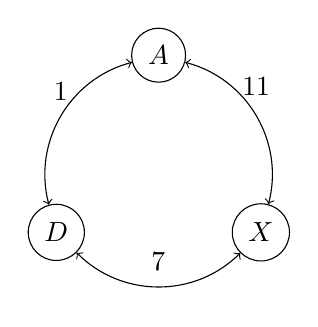
\begin{tikzpicture}[node distance=1cm, every node/.style={draw, circle, minimum height=0.1cm, minimum width=0.1cm}]
            \node (A) at (90:1.5) {$A$};
            \node (D) at (210:1.5) {$D$};
            \node (X) at (330:1.5) {$X$};
          
            \draw[<->, bend right=45] (A) to node[midway, draw=none, above] {1} (D);
            \draw[<->, bend right=45] (D) to node[midway, draw=none, above] {7} (X);
            \draw[<->, bend right=45] (X) to node[midway, draw=none, above] {11} (A);
          \end{tikzpicture}
    \end{center}
    To express this mathematically we denote the permutation represented by the Enigma at 
    position $i$ as $\sigma_i$. Since these each use the same plugboard we will also note the 
    Enigma at position $i$ not using the plugboard as $\overline{\sigma_i}$, that is $\sigma_i = P\overline{\sigma_i}P$ (conversely, $\overline\sigma_i = P\sigma_iP$).
    Then our loop is expressed by the fact that $\sigma_{11}\circ\sigma_7\circ\sigma_1$ has a fixed point at $A$. 
    We also note that the intermediate plugboard settings cancel out, that is 
    \begin{center}
        \begin{align*}
            \sigma_{1}\circ\sigma_7\circ\sigma_{11} &= P\overline{\sigma_{1}}P\circ P\overline{\sigma_7}P\circ P\overline{\sigma_{11}}P
            \\&= P\circ \overline{\sigma_{1}}\circ\overline{\sigma_7}\circ\overline{\sigma_{11}}\circ P 
        \end{align*}
    \end{center}
    We will condense this notation by defining
    \begin{center}
        $\sigma \coloneq \sigma_{1}\circ\sigma_7\circ\sigma_{11}$
    \end{center}
    and 
    \begin{center}
        $\overline{\sigma} \coloneq \overline{\sigma_{1}}\circ\overline{\sigma_7}\circ\overline{\sigma_{11}}$
    \end{center}
    And thus we have shown $\sigma = P\overline{\sigma}P$ (conversely, $\overline\sigma = P\sigma P$).
    \\\\Let us hypothesize that $A$ is steckered in the plugboard to $\alpha$ -- that is, $P(A) = \alpha$ (conversely, $P(\alpha) = A$). It then follows that for a fixed $i\in\mathbb{N}$
    \begin{center}
        \begin{align*}
            \overline{\sigma}^i(\alpha) &= P\circ\sigma^i\circ P(\alpha)
            \\&= P\circ\sigma^i(A)
            \\&= P(A)
        \end{align*}
    \end{center} 
    and so we derive 
    \begin{center}
        $P(A) = \alpha \Rightarrow P(A) = \overline{\sigma}^i(\alpha)\text{ }\forall\text{ }i\in\mathbb{N}$
    \end{center}
    Then we have that $A$ must be steckered to all values in the set $\{\overline{\sigma}^i(\alpha)\text{ }\vert\text{ }i\in\mathbb{N}\}$. 
    We note that this set is that orbit of the element $\alpha$ under the group action of the subgroup $\langle\overline{\sigma}\rangle$ -- that is, 
    $\langle\overline{\sigma}\rangle\cdot\alpha$. 
    \\\\By construction of the Enigma machine, $A$ cannot be steckered to more than one value at a time, so if $|\langle\overline{\sigma}\rangle\cdot\alpha| > 1$ our initial
    hypotheses that $P(A) = \alpha$ must have been incorrect. Further, the above argument also illustrates that $A$ cannot be steckered to any element in the orbit of $\alpha$ since 
    we would similarly find that the orbit of that element was not a singleton. Then we now have 
    \begin{center}
        $|\langle\overline{\sigma}\rangle\cdot\alpha| > 1 \Rightarrow P(A) \notin \langle\overline{\sigma}\rangle\cdot\alpha$
    \end{center} 
    thus eliminating several elements that $A$ could be steckered to. 
    \\\\By representing $\overline\sigma$ in its cycle notation we can quickly see whether certian hypotheses are possible. For example, 
    suppose we found that 
    \begin{center}
        $\overline\sigma = (ABCDEF)(GHIJK)(L)(MNOPQRSTUVWXYZ)$
    \end{center}
    If we suppose that $A$ is steckered to any element in the cycle $(ABCDEF)$ we find that this
    element has an orbit of length $6$ in $\langle\overline\sigma\rangle$ and thus $A$ cannot be steckered
    to any element in this cycle. Then it is clear that $A$ can only be steckered to $L$ in this case. 
    \subsection{Scanning Methods}
    Turing describes various methods of mechanising the above analysis of cycle-type to determine when we can eliminate rotor positions.
    \begin{enumerate}
        \item If we examine a particular hypothesis, say $A$ is steckered to $K$, we can rule out this steckering if we find that $K$ is not in a $1$-cycle, that is if $\overline\sigma(K) \ne K$. If we
        mechanize this process we can eliminate rotor positions which do not satisfy this singular hypothesis. Turing called this method \textbf{single line scanning}. Note, however, that this method may eliminate rotor
        positions which do have valid steckerings, just not the particular steckering that we hypothesized.
        \item If we perform single line scanning in sequence, that is, for each steckering hypothesis, we can rule out rotor positions which have all steckering hypotheses invalid. Turing called this method \textbf{serial scanning}.
        \item Serial scanning requires a seperate examination of each steckering. Turing proposed a machine which could concurrently examine all steckering possibilities and eliminate rotor positions
        which had no valid steckerings. Turing called this method \textbf{simultaneous scanning}.
        \item If we find $\overline\sigma$ has a $26$-cycle, then we must have that there are no $1$-cycles and thus no valid steckerings. It then follows that the rotor position is incorrect.
        If we mechanism this process we can eliminate \emph{some} rotor positions which do not have valid steckerings. We will call this method \textbf{spider scanning}. Note, however, that this method 
        would not, for example, detect that a $13,13$-cycle contains no valid steckerings. As Turing explained, 
        \say{The ideal machine that Welchman was aiming at was to reject any position in which a certain fixed-for-the-time Stecker hypothesis led to any direct contradiction... The spider does more than this in one way and 
        less in another. It is not restricted to dealing with one Stecker hypothesis at a time, and it does not find all direct contradictions.} Effectively, spider-scanning is like a form of simultaneous scanning which is restricted
        to examining only one cycle at a time.
    \end{enumerate}
    Iterations of each scanning methods were proposed or designed, but in the end we find that the spider scanning method was used in the implementation of the Bombe.At a high level, we encode the structure of the ciphertext-plaintext pairings, we input a hypothesis that a particular 
    letter (e.g $A$) is steckered to another (e.g. $\alpha$), and we electrically produce the elements that must also be steckered to our test letter 
    (e.g. $\langle\overline{\sigma}\rangle\cdot\alpha$) if our hypothesis were to be true. If we find that this production generates a set of all letters and thus disqualifies this rotor position from producing
    the plaintext we observed, then we can continue on to the next rotor position until we have no contradictory results from our hypothesis.

    \section{The Bombe}

    In the section, we outline the construction of a rudementary Bombe. Our goal is to construct a machine using the above insight to quickly elimate a rotor position based on contradictory hypotheses. For clarity sake, we will 
    imagine that our Engima machine operates on an alphabet of only four letters $\{A, B, C, D\}$.  
    We must shift from the above mathematical construction to an electrical one. We first abstract the idea of the Engima machine and do away with the input output system of keys and lamp lights.
    Rather, we imagine the Enigma machine as black-box that takes in 4 cables encoding, via current, each of the 4 letters, and outputs currents on the corresponding letter after applying the Enigma permutation.
    Imagine the following set of wires encoding a possible Enigma permutation we will denoted $\overline\sigma_\alpha$ (the bar indicates we are not yet considering the plugboard).
    
    \tikzset{big box/.style={draw, minimum width=5cm, minimum height=4cm},
    small box/.style={draw, minimum width=1cm, minimum height=1cm}}

    \begin{center}
        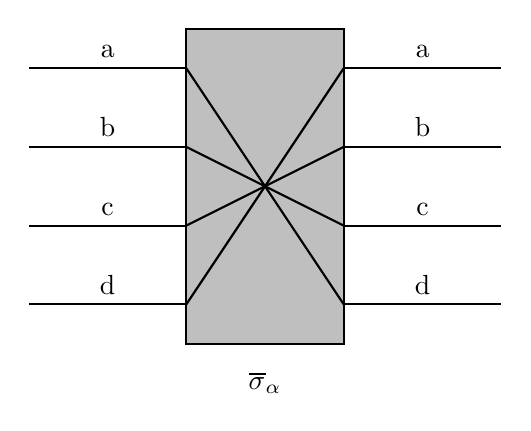
\begin{tikzpicture}[thick]
            % Draw the box
            \draw[fill=lightgray] (2,-1.5) rectangle (4,2.5) node[midway] {};
            
            \node at (3, -2) {$\overline\sigma_\alpha$};

            % Draw the wires entering the box
            \draw[-] (0, 2) -- (2, 2) node[midway, above] {a};
            \draw[-] (0, 1) -- (2, 1) node[midway, above] {b};
            \draw[-] (0, 0) -- (2, 0) node[midway, above] {c};
            \draw[-] (0,-1) -- (2,-1) node[midway, above] {d};

            % Draw the wires exiting the box with crossed mappings
            \draw[-] (4, 2) -- (6,2) node[midway, above] {a};
            \draw[-] (4, 1) -- (6, 1) node[midway, above] {b};
            \draw[-] (4, 0) -- (6, 0) node[midway, above] {c};
            \draw[-] (4,-1) -- (6, -1) node[midway, above] {d};

            % Draw the lines inside the box to represent the mapping
            \draw[-] (2, 2) -- (4,-1);
            \draw[-] (2, 1) -- (4, 0);
            \draw[-] (2, 0) -- (4, 1);
            \draw[-] (2,-1) -- (4, 2);

        \end{tikzpicture} 
    \end{center}
    A couple quick notes about this abstraction. First as these lines are simply wires, current can flow in either direction, left-to-right, or right-to-left. 
    Second, we can apply current to multiple wires concurrently, for example, applying current at $a$ and $c$ will cause $d$ and $b$ to be live on the other side of the machine.
    Finally, the choice to use lower case letters will become clear further in this section as we want to seperate the plugboard letters from the actual plaintext-ciphertext letters. 
    \\\\As described in our motivating example, we may want to connect Engima permutations in series to capture an underlying relationship between a ciphertext-plaintext pairing. 
    Suppose we had plaintext ciphertext pairing 
    \begin{center}
        \begin{tikzpicture}[node distance=1cm, every node/.style={draw, circle, minimum height=0.1cm, minimum width=0.1cm}]
        
            % Centering the diagram
            \node (a1) [] {B};
            \node (a2) [right=0.1cm of a1] {C};
            \node (a3) [right=0.1cm of a2] {A};
            
            % Nodes for ciphertext
            \node (x1) [below=1cm of a1] {A};
            \node (x2) [below=1cm of a2] {B};
            \node (x3) [below=1cm of a3] {C};
            
            % Arrows for mapping
            \draw[->] (a1) -- (x1) node[midway, left, draw=none, fill=none] {1};
            \draw[->] (a2) -- (x2) node[midway, left, draw=none, fill=none] {2};
            \draw[->] (a3) -- (x3) node[midway, left, draw=none, fill=none] {3};
            
            \end{tikzpicture}
    \end{center}

    Then we find that there exists a loop in the pairing as follows

    \begin{center}
        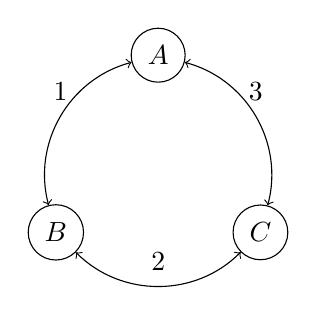
\begin{tikzpicture}[node distance=1cm, every node/.style={draw, circle, minimum height=0.1cm, minimum width=0.1cm}]
            \node (A) at (90:1.5) {$A$};
            \node (B) at (210:1.5) {$B$};
            \node (C) at (330:1.5) {$C$};
            
            \draw[<->, bend right=45] (A) to node[midway, draw=none, above] {1} (B);
            \draw[<->, bend right=45] (B) to node[midway, draw=none, above] {2} (C);
            \draw[<->, bend right=45] (C) to node[midway, draw=none, above] {3} (A);
            \end{tikzpicture}
    \end{center}
    We can then think of this loop as a series of Enigma permutations 
    \begin{center}
        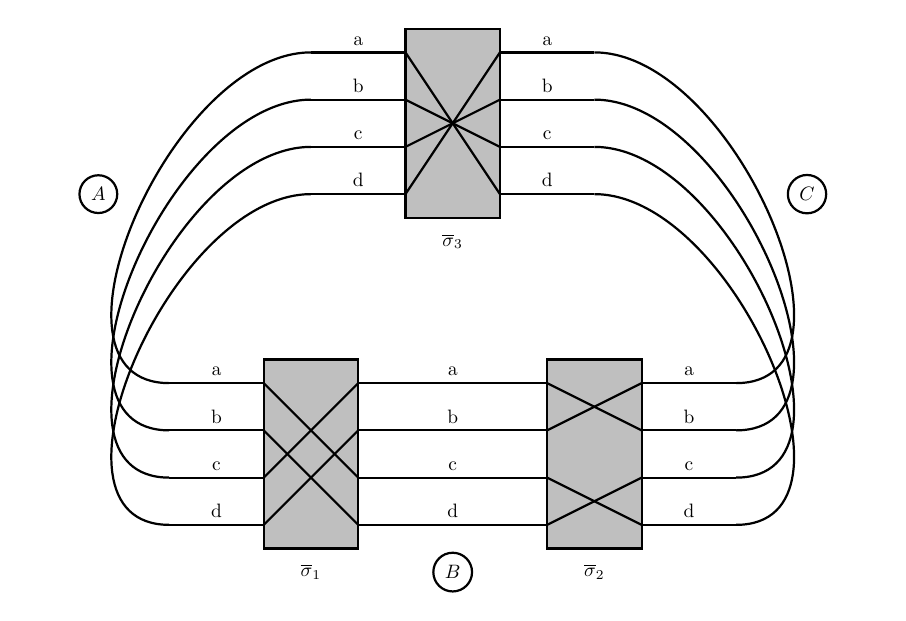
\begin{tikzpicture}[thick, scale=0.6, every node/.style={scale=0.7}]
            % Draw the box
            \draw[fill=lightgray] (2,-1.5) rectangle (4,2.5) node[midway] {};
            
            \node at (3, -2) {$\overline\sigma_3$};

            % Draw the wires entering the box
            \draw[-] (0, 2) -- (2, 2) node[midway, above] {a};
            \draw[-] (0, 1) -- (2, 1) node[midway, above] {b};
            \draw[-] (0, 0) -- (2, 0) node[midway, above] {c};
            \draw[-] (0,-1) -- (2,-1) node[midway, above] {d};

            % Draw the wires exiting the box with crossed mappings
            \draw[-] (4, 2) -- (6,2) node[midway, above] {a};
            \draw[-] (4, 1) -- (6, 1) node[midway, above] {b};
            \draw[-] (4, 0) -- (6, 0) node[midway, above] {c};
            \draw[-] (4,-1) -- (6, -1) node[midway, above] {d};

            % Draw the lines inside the box to represent the mapping
            \draw[-] (2, 2) -- (4,-1);
            \draw[-] (2, 1) -- (4, 0);
            \draw[-] (2, 0) -- (4, 1);
            \draw[-] (2,-1) -- (4, 2);

            \draw[-] (0-3, 2-7) to[out=180, in=180] (0, 2) node[midway, above] {};
            \draw[-] (0-3, 1-7) to[out=180, in=180] (0, 1) node[midway, above] {};
            \draw[-] (0-3, 0-7) to[out=180, in=180] (0, 0) node[midway, above] {};
            \draw[-] (0-3, -1-7) to[out=180, in=180] (0, -1) node[midway, above] {};

            \draw[-] (6+3, 2-7) to[out=360, in=360] (6, 2) node[midway, above] {};
            \draw[-] (6+3, 1-7) to[out=360, in=360] (6, 1) node[midway, above] {};
            \draw[-] (6+3, 0-7) to[out=360, in=360] (6, 0) node[midway, above] {};
            \draw[-] (6+3, -1-7) to[out=360, in=360] (6, -1) node[midway, above] {};

            \draw[fill=lightgray] (2-3,-1.5-7) rectangle (4-3,2.5-7) node[midway] {};

            \node at (3-3, -2-7) {$\overline\sigma_1$};

            % Draw the wires entering the box
            \draw[-] (0-3, 2-7) -- (2-3, 2-7) node[midway, above] {a};
            \draw[-] (0-3, 1-7) -- (2-3, 1-7) node[midway, above] {b};
            \draw[-] (0-3, 0-7) -- (2-3, 0-7) node[midway, above] {c};
            \draw[-] (0-3,-1-7) -- (2-3,-1-7) node[midway, above] {d};

            % Draw the wires exiting the box
            \draw[-] (4-3, 2-7) -- (6-3,2-7) node[right, above] {a};
            \draw[-] (4-3, 1-7) -- (6-3, 1-7) node[right, above] {b};
            \draw[-] (4-3, 0-7) -- (6-3, 0-7) node[right, above] {c};
            \draw[-] (4-3,-1-7) -- (6-3, -1-7) node[right, above] {d};

            % Draw the lines inside the box to represent the mapping
            \draw[-] (2-3, 2-7) -- (4-3, 0-7);
            \draw[-] (2-3, 1-7) -- (4-3, -1-7);
            \draw[-] (2-3, 0-7) -- (4-3, 2-7);
            \draw[-] (2-3,-1-7) -- (4-3, 1-7);

            \draw[fill=lightgray] (2+3,-1.5-7) rectangle (4+3,2.5-7) node[midway] {};
            
            \node at (3+3, -2-7) {$\overline\sigma_2$};


            % Draw the wires entering the box
            \draw[-] (0+3, 2-7) -- (2+3, 2-7) node[midway, above] {};
            \draw[-] (0+3, 1-7) -- (2+3, 1-7) node[midway, above] {};
            \draw[-] (0+3, 0-7) -- (2+3, 0-7) node[midway, above] {};
            \draw[-] (0+3,-1-7) -- (2+3,-1-7) node[midway, above] {};

            % Draw the wires exiting the box
            \draw[-] (4+3, 2-7) -- (6+3,2-7) node[midway, above] {a};
            \draw[-] (4+3, 1-7) -- (6+3, 1-7) node[midway, above] {b};
            \draw[-] (4+3, 0-7) -- (6+3, 0-7) node[midway, above] {c};
            \draw[-] (4+3,-1-7) -- (6+3, -1-7) node[midway, above] {d};

            \draw[-] (2+3, 2-7) -- (4+3, 1-7);
            \draw[-] (2+3, 1-7) -- (4+3, 2-7);
            \draw[-] (2+3, 0-7) -- (4+3, -1-7);
            \draw[-] (2+3,-1-7) -- (4+3, 0-7);

            \node[draw,circle] at (-4.5, -1) {$A$};
            \node[draw,circle] at (3, -9) {$B$};
            \node[draw,circle] at (10.5, -1) {$C$};



        \end{tikzpicture}
    \end{center}
    As before, let us make a hypothesis regarding steckering. Suppose $P(A) = D$. We know that $A$ must map to $A$ via 
    $P\overline\sigma_3\overline\sigma_2\overline\sigma_1 P$. In our diagram, however we do not see a plugboard so how can we represent the plugboard's involvement? In order 
    to achieve this \emph{we} will function as the plugboard by applying voltage to the $d$ line on the $A$ thus implicitly performing the plugboard mapping in which $P(A) = D$. 
    Then this will go through the electrical mapping $\overline\sigma_1$ arriving on the $B$ cable, followed by $\overline\sigma_2$ arriving on the $C$ cable, followed by $\overline\sigma_3$ arriving back on the $A$ cable, where \emph{we} as the implicit plugboard know that 
    the output of this electrical mapping must go through the pluboard again to get a final output of $A$.
    \\\\We will denote each wire by a capital and lowercase letter which indicates both the cable and specific wire to which we refer. For instance, line $d$ on cable $A$ will be denoted $Ad$. Any time a wire 
    $Xy$ is live, implicitly this means that there is an intermediary plugboard which mapped $P(X) = Y$ or $P(Y) = X$. 
    To see this electrical mapping occur let us visualize a current being sent through $Ad$.
    \begin{center}
        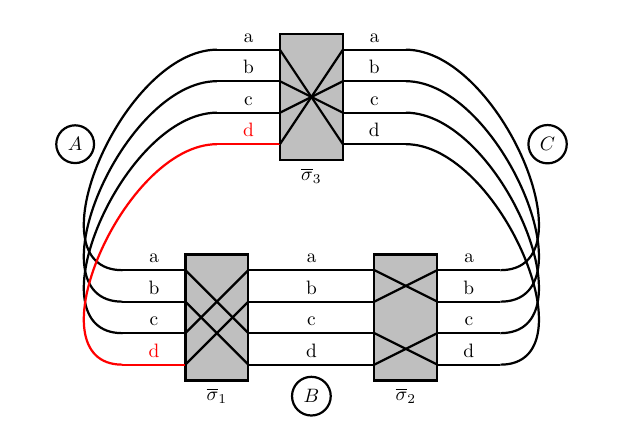
\begin{tikzpicture}[thick, scale=0.4, every node/.style={scale=0.7}]
            % Draw the box
            \draw[fill=lightgray] (2,-1.5) rectangle (4,2.5) node[midway] {};
            
            \node at (3, -2) {$\overline\sigma_3$};

            % Draw the wires entering the box
            \draw[-] (0, 2) -- (2, 2) node[midway, above] {a};
            \draw[-] (0, 1) -- (2, 1) node[midway, above] {b};
            \draw[-] (0, 0) -- (2, 0) node[midway, above] {c};
            \draw[-, red] (0,-1) -- (2,-1) node[midway, above] {d};

            % Draw the wires exiting the box with crossed mappings
            \draw[-] (4, 2) -- (6,2) node[midway, above] {a};
            \draw[-] (4, 1) -- (6, 1) node[midway, above] {b};
            \draw[-] (4, 0) -- (6, 0) node[midway, above] {c};
            \draw[-] (4,-1) -- (6, -1) node[midway, above] {d};

            % Draw the lines inside the box to represent the mapping
            \draw[-] (2, 2) -- (4,-1);
            \draw[-] (2, 1) -- (4, 0);
            \draw[-] (2, 0) -- (4, 1);
            \draw[-] (2,-1) -- (4, 2);

            \draw[-] (0-3, 2-7) to[out=180, in=180] (0, 2) node[midway, above] {};
            \draw[-] (0-3, 1-7) to[out=180, in=180] (0, 1) node[midway, above] {};
            \draw[-] (0-3, 0-7) to[out=180, in=180] (0, 0) node[midway, above] {};
            \draw[-, red] (0-3, -1-7) to[out=180, in=180] (0, -1) node[midway, above] {};

            \draw[-] (6+3, 2-7) to[out=360, in=360] (6, 2) node[midway, above] {};
            \draw[-] (6+3, 1-7) to[out=360, in=360] (6, 1) node[midway, above] {};
            \draw[-] (6+3, 0-7) to[out=360, in=360] (6, 0) node[midway, above] {};
            \draw[-] (6+3, -1-7) to[out=360, in=360] (6, -1) node[midway, above] {};

            \draw[fill=lightgray] (2-3,-1.5-7) rectangle (4-3,2.5-7) node[midway] {};

            \node at (3-3, -2-7) {$\overline\sigma_1$};

            % Draw the wires entering the box
            \draw[-] (0-3, 2-7) -- (2-3, 2-7) node[midway, above] {a};
            \draw[-] (0-3, 1-7) -- (2-3, 1-7) node[midway, above] {b};
            \draw[-] (0-3, 0-7) -- (2-3, 0-7) node[midway, above] {c};
            \draw[-, red] (0-3,-1-7) -- (2-3,-1-7) node[midway, above] {d};

            % Draw the wires exiting the box
            \draw[-] (4-3, 2-7) -- (6-3,2-7) node[right, above] {a};
            \draw[-] (4-3, 1-7) -- (6-3, 1-7) node[right, above] {b};
            \draw[-] (4-3, 0-7) -- (6-3, 0-7) node[right, above] {c};
            \draw[-] (4-3,-1-7) -- (6-3, -1-7) node[right, above] {d};

            % Draw the lines inside the box to represent the mapping
            \draw[-] (2-3, 2-7) -- (4-3, 0-7);
            \draw[-] (2-3, 1-7) -- (4-3, -1-7);
            \draw[-] (2-3, 0-7) -- (4-3, 2-7);
            \draw[-] (2-3,-1-7) -- (4-3, 1-7);

            \draw[fill=lightgray] (2+3,-1.5-7) rectangle (4+3,2.5-7) node[midway] {};
            
            \node at (3+3, -2-7) {$\overline\sigma_2$};


            % Draw the wires entering the box
            \draw[-] (0+3, 2-7) -- (2+3, 2-7) node[midway, above] {};
            \draw[-] (0+3, 1-7) -- (2+3, 1-7) node[midway, above] {};
            \draw[-] (0+3, 0-7) -- (2+3, 0-7) node[midway, above] {};
            \draw[-] (0+3,-1-7) -- (2+3,-1-7) node[midway, above] {};

            % Draw the wires exiting the box
            \draw[-] (4+3, 2-7) -- (6+3,2-7) node[midway, above] {a};
            \draw[-] (4+3, 1-7) -- (6+3, 1-7) node[midway, above] {b};
            \draw[-] (4+3, 0-7) -- (6+3, 0-7) node[midway, above] {c};
            \draw[-] (4+3,-1-7) -- (6+3, -1-7) node[midway, above] {d};

            \draw[-] (2+3, 2-7) -- (4+3, 1-7);
            \draw[-] (2+3, 1-7) -- (4+3, 2-7);
            \draw[-] (2+3, 0-7) -- (4+3, -1-7);
            \draw[-] (2+3,-1-7) -- (4+3, 0-7);

            \node[draw,circle] at (-4.5, -1) {$A$};
            \node[draw,circle] at (3, -9) {$B$};
            \node[draw,circle] at (10.5, -1) {$C$};



        \end{tikzpicture}
    \end{center}
    \begin{center}
        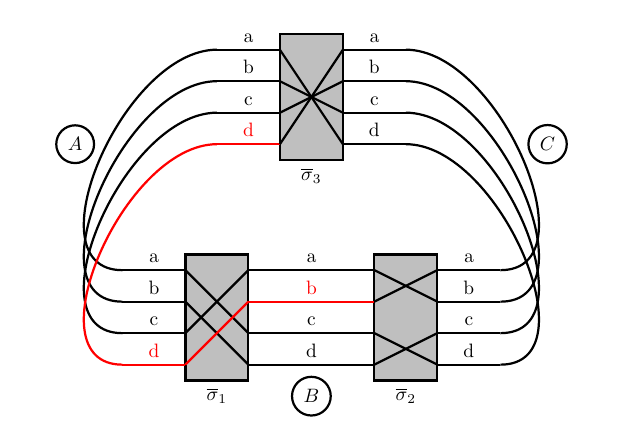
\begin{tikzpicture}[thick, scale=0.4, every node/.style={scale=0.7}]
            % Draw the box
            \draw[fill=lightgray] (2,-1.5) rectangle (4,2.5) node[midway] {};
            
            \node at (3, -2) {$\overline\sigma_3$};

            % Draw the wires entering the box
            \draw[-] (0, 2) -- (2, 2) node[midway, above] {a};
            \draw[-] (0, 1) -- (2, 1) node[midway, above] {b};
            \draw[-] (0, 0) -- (2, 0) node[midway, above] {c};
            \draw[-, red] (0,-1) -- (2,-1) node[midway, above] {d};

            % Draw the wires exiting the box with crossed mappings
            \draw[-] (4, 2) -- (6,2) node[midway, above] {a};
            \draw[-] (4, 1) -- (6, 1) node[midway, above] {b};
            \draw[-] (4, 0) -- (6, 0) node[midway, above] {c};
            \draw[-] (4,-1) -- (6, -1) node[midway, above] {d};

            % Draw the lines inside the box to represent the mapping
            \draw[-] (2, 2) -- (4,-1);
            \draw[-] (2, 1) -- (4, 0);
            \draw[-] (2, 0) -- (4, 1);
            \draw[-] (2,-1) -- (4, 2);

            \draw[-] (0-3, 2-7) to[out=180, in=180] (0, 2) node[midway, above] {};
            \draw[-] (0-3, 1-7) to[out=180, in=180] (0, 1) node[midway, above] {};
            \draw[-] (0-3, 0-7) to[out=180, in=180] (0, 0) node[midway, above] {};
            \draw[-, red] (0-3, -1-7) to[out=180, in=180] (0, -1) node[midway, above] {};

            \draw[-] (6+3, 2-7) to[out=360, in=360] (6, 2) node[midway, above] {};
            \draw[-] (6+3, 1-7) to[out=360, in=360] (6, 1) node[midway, above] {};
            \draw[-] (6+3, 0-7) to[out=360, in=360] (6, 0) node[midway, above] {};
            \draw[-] (6+3, -1-7) to[out=360, in=360] (6, -1) node[midway, above] {};

            \draw[fill=lightgray] (2-3,-1.5-7) rectangle (4-3,2.5-7) node[midway] {};

            \node at (3-3, -2-7) {$\overline\sigma_1$};

            % Draw the wires entering the box
            \draw[-] (0-3, 2-7) -- (2-3, 2-7) node[midway, above] {a};
            \draw[-] (0-3, 1-7) -- (2-3, 1-7) node[midway, above] {b};
            \draw[-] (0-3, 0-7) -- (2-3, 0-7) node[midway, above] {c};
            \draw[-, red] (0-3,-1-7) -- (2-3,-1-7) node[midway, above] {d};

            % Draw the wires exiting the box
            \draw[-] (4-3, 2-7) -- (6-3,2-7) node[right, above] {a};
            \draw[-, red] (4-3, 1-7) -- (6-3, 1-7) node[right, above] {b};
            \draw[-] (4-3, 0-7) -- (6-3, 0-7) node[right, above] {c};
            \draw[-] (4-3,-1-7) -- (6-3, -1-7) node[right, above] {d};

            % Draw the lines inside the box to represent the mapping
            \draw[-] (2-3, 2-7) -- (4-3, 0-7);
            \draw[-] (2-3, 1-7) -- (4-3, -1-7);
            \draw[-] (2-3, 0-7) -- (4-3, 2-7);
            \draw[-, red] (2-3,-1-7) -- (4-3, 1-7);

            \draw[fill=lightgray] (2+3,-1.5-7) rectangle (4+3,2.5-7) node[midway] {};
            
            \node at (3+3, -2-7) {$\overline\sigma_2$};


            % Draw the wires entering the box
            \draw[-] (0+3, 2-7) -- (2+3, 2-7) node[midway, above] {};
            \draw[-, red] (0+3, 1-7) -- (2+3, 1-7) node[midway, above] {};
            \draw[-] (0+3, 0-7) -- (2+3, 0-7) node[midway, above] {};
            \draw[-] (0+3,-1-7) -- (2+3,-1-7) node[midway, above] {};

            % Draw the wires exiting the box
            \draw[-] (4+3, 2-7) -- (6+3,2-7) node[midway, above] {a};
            \draw[-] (4+3, 1-7) -- (6+3, 1-7) node[midway, above] {b};
            \draw[-] (4+3, 0-7) -- (6+3, 0-7) node[midway, above] {c};
            \draw[-] (4+3,-1-7) -- (6+3, -1-7) node[midway, above] {d};

            \draw[-] (2+3, 2-7) -- (4+3, 1-7);
            \draw[-] (2+3, 1-7) -- (4+3, 2-7);
            \draw[-] (2+3, 0-7) -- (4+3, -1-7);
            \draw[-] (2+3,-1-7) -- (4+3, 0-7);

            \node[draw,circle] at (-4.5, -1) {$A$};
            \node[draw,circle] at (3, -9) {$B$};
            \node[draw,circle] at (10.5, -1) {$C$};



        \end{tikzpicture}
    \end{center}
    \begin{center}
        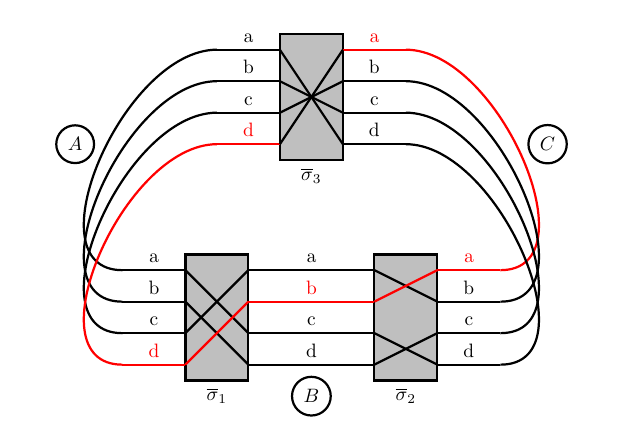
\begin{tikzpicture}[thick, scale=0.4, every node/.style={scale=0.7}]
            % Draw the box
            \draw[fill=lightgray] (2,-1.5) rectangle (4,2.5) node[midway] {};
            
            \node at (3, -2) {$\overline\sigma_3$};

            % Draw the wires entering the box
            \draw[-] (0, 2) -- (2, 2) node[midway, above] {a};
            \draw[-] (0, 1) -- (2, 1) node[midway, above] {b};
            \draw[-] (0, 0) -- (2, 0) node[midway, above] {c};
            \draw[-, red] (0,-1) -- (2,-1) node[midway, above] {d};

            % Draw the wires exiting the box with crossed mappings
            \draw[-, red] (4, 2) -- (6,2) node[midway, above] {a};
            \draw[-] (4, 1) -- (6, 1) node[midway, above] {b};
            \draw[-] (4, 0) -- (6, 0) node[midway, above] {c};
            \draw[-] (4,-1) -- (6, -1) node[midway, above] {d};

            % Draw the lines inside the box to represent the mapping
            \draw[-] (2, 2) -- (4,-1);
            \draw[-] (2, 1) -- (4, 0);
            \draw[-] (2, 0) -- (4, 1);
            \draw[-] (2,-1) -- (4, 2);

            \draw[-] (0-3, 2-7) to[out=180, in=180] (0, 2) node[midway, above] {};
            \draw[-] (0-3, 1-7) to[out=180, in=180] (0, 1) node[midway, above] {};
            \draw[-] (0-3, 0-7) to[out=180, in=180] (0, 0) node[midway, above] {};
            \draw[-, red] (0-3, -1-7) to[out=180, in=180] (0, -1) node[midway, above] {};

            \draw[- ,red] (6+3, 2-7) to[out=360, in=360] (6, 2) node[midway, above] {};
            \draw[-] (6+3, 1-7) to[out=360, in=360] (6, 1) node[midway, above] {};
            \draw[-] (6+3, 0-7) to[out=360, in=360] (6, 0) node[midway, above] {};
            \draw[-] (6+3, -1-7) to[out=360, in=360] (6, -1) node[midway, above] {};

            \draw[fill=lightgray] (2-3,-1.5-7) rectangle (4-3,2.5-7) node[midway] {};

            \node at (3-3, -2-7) {$\overline\sigma_1$};

            % Draw the wires entering the box
            \draw[-] (0-3, 2-7) -- (2-3, 2-7) node[midway, above] {a};
            \draw[-] (0-3, 1-7) -- (2-3, 1-7) node[midway, above] {b};
            \draw[-] (0-3, 0-7) -- (2-3, 0-7) node[midway, above] {c};
            \draw[-, red] (0-3,-1-7) -- (2-3,-1-7) node[midway, above] {d};

            % Draw the wires exiting the box
            \draw[-] (4-3, 2-7) -- (6-3,2-7) node[right, above] {a};
            \draw[-, red] (4-3, 1-7) -- (6-3, 1-7) node[right, above] {b};
            \draw[-] (4-3, 0-7) -- (6-3, 0-7) node[right, above] {c};
            \draw[-] (4-3,-1-7) -- (6-3, -1-7) node[right, above] {d};

            % Draw the lines inside the box to represent the mapping
            \draw[-] (2-3, 2-7) -- (4-3, 0-7);
            \draw[-] (2-3, 1-7) -- (4-3, -1-7);
            \draw[-] (2-3, 0-7) -- (4-3, 2-7);
            \draw[-, red] (2-3,-1-7) -- (4-3, 1-7);

            \draw[fill=lightgray] (2+3,-1.5-7) rectangle (4+3,2.5-7) node[midway] {};
            
            \node at (3+3, -2-7) {$\overline\sigma_2$};


            % Draw the wires entering the box
            \draw[-] (0+3, 2-7) -- (2+3, 2-7) node[midway, above] {};
            \draw[-, red] (0+3, 1-7) -- (2+3, 1-7) node[midway, above] {};
            \draw[-] (0+3, 0-7) -- (2+3, 0-7) node[midway, above] {};
            \draw[-] (0+3,-1-7) -- (2+3,-1-7) node[midway, above] {};

            % Draw the wires exiting the box
            \draw[-, red] (4+3, 2-7) -- (6+3,2-7) node[midway, above] {a};
            \draw[-] (4+3, 1-7) -- (6+3, 1-7) node[midway, above] {b};
            \draw[-] (4+3, 0-7) -- (6+3, 0-7) node[midway, above] {c};
            \draw[-] (4+3,-1-7) -- (6+3, -1-7) node[midway, above] {d};

            \draw[-] (2+3, 2-7) -- (4+3, 1-7);
            \draw[-, red] (2+3, 1-7) -- (4+3, 2-7);
            \draw[-] (2+3, 0-7) -- (4+3, -1-7);
            \draw[-] (2+3,-1-7) -- (4+3, 0-7);

            \node[draw,circle] at (-4.5, -1) {$A$};
            \node[draw,circle] at (3, -9) {$B$};
            \node[draw,circle] at (10.5, -1) {$C$};



        \end{tikzpicture}
    \end{center}

    \begin{center}
        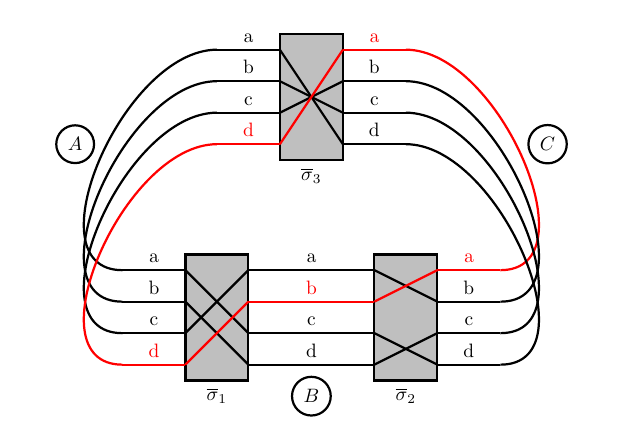
\begin{tikzpicture}[thick, scale=0.4, every node/.style={scale=0.7}]
            % Draw the box
            \draw[fill=lightgray] (2,-1.5) rectangle (4,2.5) node[midway] {};
            
            \node at (3, -2) {$\overline\sigma_3$};

            % Draw the wires entering the box
            \draw[-] (0, 2) -- (2, 2) node[midway, above] {a};
            \draw[-] (0, 1) -- (2, 1) node[midway, above] {b};
            \draw[-] (0, 0) -- (2, 0) node[midway, above] {c};
            \draw[-, red] (0,-1) -- (2,-1) node[midway, above] {d};

            % Draw the wires exiting the box with crossed mappings
            \draw[-, red] (4, 2) -- (6,2) node[midway, above] {a};
            \draw[-] (4, 1) -- (6, 1) node[midway, above] {b};
            \draw[-] (4, 0) -- (6, 0) node[midway, above] {c};
            \draw[-] (4,-1) -- (6, -1) node[midway, above] {d};

            % Draw the lines inside the box to represent the mapping
            \draw[-] (2, 2) -- (4,-1);
            \draw[-] (2, 1) -- (4, 0);
            \draw[-] (2, 0) -- (4, 1);
            \draw[-, red] (2,-1) -- (4, 2);

            \draw[-] (0-3, 2-7) to[out=180, in=180] (0, 2) node[midway, above] {};
            \draw[-] (0-3, 1-7) to[out=180, in=180] (0, 1) node[midway, above] {};
            \draw[-] (0-3, 0-7) to[out=180, in=180] (0, 0) node[midway, above] {};
            \draw[-, red] (0-3, -1-7) to[out=180, in=180] (0, -1) node[midway, above] {};

            \draw[- ,red] (6+3, 2-7) to[out=360, in=360] (6, 2) node[midway, above] {};
            \draw[-] (6+3, 1-7) to[out=360, in=360] (6, 1) node[midway, above] {};
            \draw[-] (6+3, 0-7) to[out=360, in=360] (6, 0) node[midway, above] {};
            \draw[-] (6+3, -1-7) to[out=360, in=360] (6, -1) node[midway, above] {};

            \draw[fill=lightgray] (2-3,-1.5-7) rectangle (4-3,2.5-7) node[midway] {};

            \node at (3-3, -2-7) {$\overline\sigma_1$};

            % Draw the wires entering the box
            \draw[-] (0-3, 2-7) -- (2-3, 2-7) node[midway, above] {a};
            \draw[-] (0-3, 1-7) -- (2-3, 1-7) node[midway, above] {b};
            \draw[-] (0-3, 0-7) -- (2-3, 0-7) node[midway, above] {c};
            \draw[-, red] (0-3,-1-7) -- (2-3,-1-7) node[midway, above] {d};

            % Draw the wires exiting the box
            \draw[-] (4-3, 2-7) -- (6-3,2-7) node[right, above] {a};
            \draw[-, red] (4-3, 1-7) -- (6-3, 1-7) node[right, above] {b};
            \draw[-] (4-3, 0-7) -- (6-3, 0-7) node[right, above] {c};
            \draw[-] (4-3,-1-7) -- (6-3, -1-7) node[right, above] {d};

            % Draw the lines inside the box to represent the mapping
            \draw[-] (2-3, 2-7) -- (4-3, 0-7);
            \draw[-] (2-3, 1-7) -- (4-3, -1-7);
            \draw[-] (2-3, 0-7) -- (4-3, 2-7);
            \draw[-, red] (2-3,-1-7) -- (4-3, 1-7);

            \draw[fill=lightgray] (2+3,-1.5-7) rectangle (4+3,2.5-7) node[midway] {};
            
            \node at (3+3, -2-7) {$\overline\sigma_2$};


            % Draw the wires entering the box
            \draw[-] (0+3, 2-7) -- (2+3, 2-7) node[midway, above] {};
            \draw[-, red] (0+3, 1-7) -- (2+3, 1-7) node[midway, above] {};
            \draw[-] (0+3, 0-7) -- (2+3, 0-7) node[midway, above] {};
            \draw[-] (0+3,-1-7) -- (2+3,-1-7) node[midway, above] {};

            % Draw the wires exiting the box
            \draw[-, red] (4+3, 2-7) -- (6+3,2-7) node[midway, above] {a};
            \draw[-] (4+3, 1-7) -- (6+3, 1-7) node[midway, above] {b};
            \draw[-] (4+3, 0-7) -- (6+3, 0-7) node[midway, above] {c};
            \draw[-] (4+3,-1-7) -- (6+3, -1-7) node[midway, above] {d};

            \draw[-] (2+3, 2-7) -- (4+3, 1-7);
            \draw[-, red] (2+3, 1-7) -- (4+3, 2-7);
            \draw[-] (2+3, 0-7) -- (4+3, -1-7);
            \draw[-] (2+3,-1-7) -- (4+3, 0-7);

            \node[draw,circle] at (-4.5, -1) {$A$};
            \node[draw,circle] at (3, -9) {$B$};
            \node[draw,circle] at (10.5, -1) {$C$};



        \end{tikzpicture}
    \end{center}
    Following our hypothesis that $P(A) = D$ we find that after sending current through $Ad$ we arrive after mapping through $\overline\sigma$ back at $Ad$ and this makes sense since we know that
    $D$ will map back to $A$ thus preserving the loop in our ciphertext-plaintext pairing. On the other hand, if we change $\overline\sigma$ and repreat this process which may end up in the following sitatuation 
    \begin{center}
        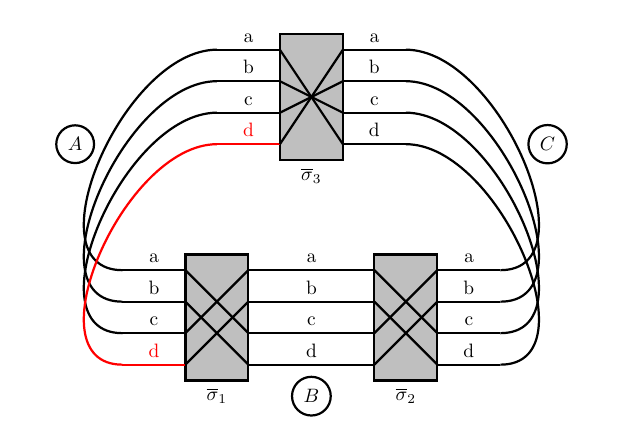
\begin{tikzpicture}[thick, scale=0.4, every node/.style={scale=0.7}]
            % Draw the box
            \draw[fill=lightgray] (2,-1.5) rectangle (4,2.5) node[midway] {};
            
            \node at (3, -2) {$\overline\sigma_3$};

            % Draw the wires entering the box
            \draw[-] (0, 2) -- (2, 2) node[midway, above] {a};
            \draw[-] (0, 1) -- (2, 1) node[midway, above] {b};
            \draw[-] (0, 0) -- (2, 0) node[midway, above] {c};
            \draw[-, red] (0,-1) -- (2,-1) node[midway, above] {d};

            % Draw the wires exiting the box with crossed mappings
            \draw[-] (4, 2) -- (6,2) node[midway, above] {a};
            \draw[-] (4, 1) -- (6, 1) node[midway, above] {b};
            \draw[-] (4, 0) -- (6, 0) node[midway, above] {c};
            \draw[-] (4,-1) -- (6, -1) node[midway, above] {d};

            % Draw the lines inside the box to represent the mapping
            \draw[-] (2, 2) -- (4,-1);
            \draw[-] (2, 1) -- (4, 0);
            \draw[-] (2, 0) -- (4, 1);
            \draw[-] (2,-1) -- (4, 2);

            \draw[-] (0-3, 2-7) to[out=180, in=180] (0, 2) node[midway, above] {};
            \draw[-] (0-3, 1-7) to[out=180, in=180] (0, 1) node[midway, above] {};
            \draw[-] (0-3, 0-7) to[out=180, in=180] (0, 0) node[midway, above] {};
            \draw[-, red] (0-3, -1-7) to[out=180, in=180] (0, -1) node[midway, above] {};

            \draw[-] (6+3, 2-7) to[out=360, in=360] (6, 2) node[midway, above] {};
            \draw[-] (6+3, 1-7) to[out=360, in=360] (6, 1) node[midway, above] {};
            \draw[-] (6+3, 0-7) to[out=360, in=360] (6, 0) node[midway, above] {};
            \draw[-] (6+3, -1-7) to[out=360, in=360] (6, -1) node[midway, above] {};

            \draw[fill=lightgray] (2-3,-1.5-7) rectangle (4-3,2.5-7) node[midway] {};

            \node at (3-3, -2-7) {$\overline\sigma_1$};

            % Draw the wires entering the box
            \draw[-] (0-3, 2-7) -- (2-3, 2-7) node[midway, above] {a};
            \draw[-] (0-3, 1-7) -- (2-3, 1-7) node[midway, above] {b};
            \draw[-] (0-3, 0-7) -- (2-3, 0-7) node[midway, above] {c};
            \draw[-, red] (0-3,-1-7) -- (2-3,-1-7) node[midway, above] {d};

            % Draw the wires exiting the box
            \draw[-] (4-3, 2-7) -- (6-3,2-7) node[right, above] {a};
            \draw[-] (4-3, 1-7) -- (6-3, 1-7) node[right, above] {b};
            \draw[-] (4-3, 0-7) -- (6-3, 0-7) node[right, above] {c};
            \draw[-] (4-3,-1-7) -- (6-3, -1-7) node[right, above] {d};

            % Draw the lines inside the box to represent the mapping
            \draw[-] (2-3, 2-7) -- (4-3, 0-7);
            \draw[-] (2-3, 1-7) -- (4-3, -1-7);
            \draw[-] (2-3, 0-7) -- (4-3, 2-7);
            \draw[-] (2-3,-1-7) -- (4-3, 1-7);

            \draw[fill=lightgray] (2+3,-1.5-7) rectangle (4+3,2.5-7) node[midway] {};
            
            \node at (3+3, -2-7) {$\overline\sigma_2$};


            % Draw the wires entering the box
            \draw[-] (0+3, 2-7) -- (2+3, 2-7) node[midway, above] {};
            \draw[-] (0+3, 1-7) -- (2+3, 1-7) node[midway, above] {};
            \draw[-] (0+3, 0-7) -- (2+3, 0-7) node[midway, above] {};
            \draw[-] (0+3,-1-7) -- (2+3,-1-7) node[midway, above] {};

            % Draw the wires exiting the box
            \draw[-] (4+3, 2-7) -- (6+3,2-7) node[midway, above] {a};
            \draw[-] (4+3, 1-7) -- (6+3, 1-7) node[midway, above] {b};
            \draw[-] (4+3, 0-7) -- (6+3, 0-7) node[midway, above] {c};
            \draw[-] (4+3,-1-7) -- (6+3, -1-7) node[midway, above] {d};

            \draw[-] (2+3, 2-7) -- (4+3, 0-7);
            \draw[-] (2+3, 1-7) -- (4+3, -1-7);
            \draw[-] (2+3, 0-7) -- (4+3, 2-7);
            \draw[-] (2+3,-1-7) -- (4+3, 1-7);

            \node[draw,circle] at (-4.5, -1) {$A$};
            \node[draw,circle] at (3, -9) {$B$};
            \node[draw,circle] at (10.5, -1) {$C$};

        \end{tikzpicture}
    \end{center}
    \begin{center}
        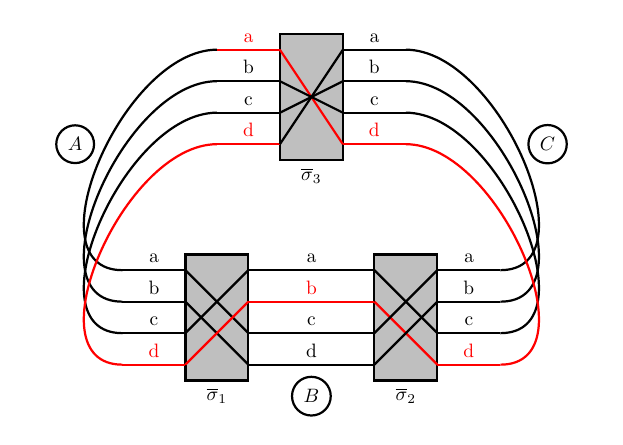
\begin{tikzpicture}[thick, scale=0.4, every node/.style={scale=0.7}]
            % Draw the box
            \draw[fill=lightgray] (2,-1.5) rectangle (4,2.5) node[midway] {};
            
            \node at (3, -2) {$\overline\sigma_3$};

            % Draw the wires entering the box
            \draw[-, red] (0, 2) -- (2, 2) node[midway, above] {a};
            \draw[-] (0, 1) -- (2, 1) node[midway, above] {b};
            \draw[-] (0, 0) -- (2, 0) node[midway, above] {c};
            \draw[-, red] (0,-1) -- (2,-1) node[midway, above] {d};

            % Draw the wires exiting the box with crossed mappings
            \draw[-] (4, 2) -- (6,2) node[midway, above] {a};
            \draw[-] (4, 1) -- (6, 1) node[midway, above] {b};
            \draw[-] (4, 0) -- (6, 0) node[midway, above] {c};
            \draw[-, red] (4,-1) -- (6, -1) node[midway, above] {d};

            % Draw the lines inside the box to represent the mapping
            \draw[-, red] (2, 2) -- (4,-1);
            \draw[-] (2, 1) -- (4, 0);
            \draw[-] (2, 0) -- (4, 1);
            \draw[-] (2,-1) -- (4, 2);

            \draw[-] (0-3, 2-7) to[out=180, in=180] (0, 2) node[midway, above] {};
            \draw[-] (0-3, 1-7) to[out=180, in=180] (0, 1) node[midway, above] {};
            \draw[-] (0-3, 0-7) to[out=180, in=180] (0, 0) node[midway, above] {};
            \draw[-, red] (0-3, -1-7) to[out=180, in=180] (0, -1) node[midway, above] {};

            \draw[-] (6+3, 2-7) to[out=360, in=360] (6, 2) node[midway, above] {};
            \draw[-] (6+3, 1-7) to[out=360, in=360] (6, 1) node[midway, above] {};
            \draw[-] (6+3, 0-7) to[out=360, in=360] (6, 0) node[midway, above] {};
            \draw[-, red] (6+3, -1-7) to[out=360, in=360] (6, -1) node[midway, above] {};

            \draw[fill=lightgray] (2-3,-1.5-7) rectangle (4-3,2.5-7) node[midway] {};

            \node at (3-3, -2-7) {$\overline\sigma_1$};

            % Draw the wires entering the box
            \draw[-] (0-3, 2-7) -- (2-3, 2-7) node[midway, above] {a};
            \draw[-] (0-3, 1-7) -- (2-3, 1-7) node[midway, above] {b};
            \draw[-] (0-3, 0-7) -- (2-3, 0-7) node[midway, above] {c};
            \draw[-, red] (0-3,-1-7) -- (2-3,-1-7) node[midway, above] {d};

            % Draw the wires exiting the box
            \draw[-] (4-3, 2-7) -- (6-3,2-7) node[right, above] {a};
            \draw[-, red] (4-3, 1-7) -- (6-3, 1-7) node[right, above] {b};
            \draw[-] (4-3, 0-7) -- (6-3, 0-7) node[right, above] {c};
            \draw[-] (4-3,-1-7) -- (6-3, -1-7) node[right, above] {d};

            % Draw the lines inside the box to represent the mapping
            \draw[-] (2-3, 2-7) -- (4-3, 0-7);
            \draw[-] (2-3, 1-7) -- (4-3, -1-7);
            \draw[-] (2-3, 0-7) -- (4-3, 2-7);
            \draw[-, red] (2-3,-1-7) -- (4-3, 1-7);

            \draw[fill=lightgray] (2+3,-1.5-7) rectangle (4+3,2.5-7) node[midway] {};
            
            \node at (3+3, -2-7) {$\overline\sigma_2$};


            % Draw the wires entering the box
            \draw[-] (0+3, 2-7) -- (2+3, 2-7) node[midway, above] {};
            \draw[-, red] (0+3, 1-7) -- (2+3, 1-7) node[midway, above] {};
            \draw[-] (0+3, 0-7) -- (2+3, 0-7) node[midway, above] {};
            \draw[-] (0+3,-1-7) -- (2+3,-1-7) node[midway, above] {};

            % Draw the wires exiting the box
            \draw[-] (4+3, 2-7) -- (6+3,2-7) node[midway, above] {a};
            \draw[-] (4+3, 1-7) -- (6+3, 1-7) node[midway, above] {b};
            \draw[-] (4+3, 0-7) -- (6+3, 0-7) node[midway, above] {c};
            \draw[-, red] (4+3,-1-7) -- (6+3, -1-7) node[midway, above] {d};

            \draw[-] (2+3, 2-7) -- (4+3, 0-7);
            \draw[-, red] (2+3, 1-7) -- (4+3, -1-7);
            \draw[-] (2+3, 0-7) -- (4+3, 2-7);
            \draw[-] (2+3,-1-7) -- (4+3, 1-7);

            \node[draw,circle] at (-4.5, -1) {$A$};
            \node[draw,circle] at (3, -9) {$B$};
            \node[draw,circle] at (10.5, -1) {$C$};

        \end{tikzpicture}
    \end{center}

    In this example, following our steckering hypothesis $P(A) = D$, results in $Aa$ becoming live after mapping through $\overline\sigma$ and 
    thus we must have $P(A) = A$ as well in order for this to ultimately map back to $A$ and preserve our ciphertext-plaintext loop above. Thus we can eliminate the steckering possibilities that 
    $P(A) \in \{A, D\}$. Effectively, this process is a mechanization of finding the cycle containing a particular letter. In the above diagram sending current from $Ad$ until we arrive back at $Ad$ is akin to repeatedly applying $\overline\sigma$ to $D$ 
    until we return to $D$. This can be visualized in our diagram as 

    \begin{center}
        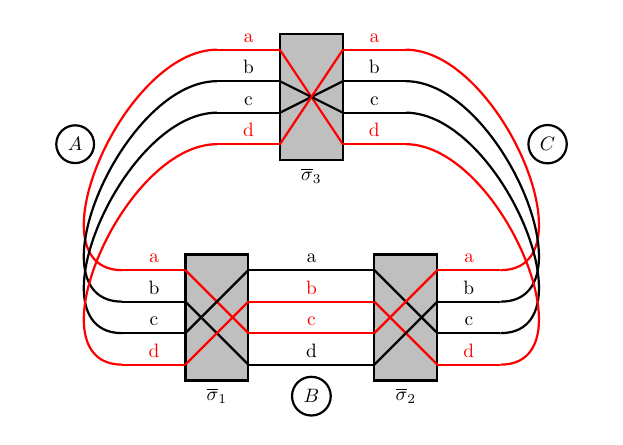
\begin{tikzpicture}[thick, scale=0.4, every node/.style={scale=0.7}]
            % Draw the box
            \draw[fill=lightgray] (2,-1.5) rectangle (4,2.5) node[midway] {};
            
            \node at (3, -2) {$\overline\sigma_3$};

            % Draw the wires entering the box
            \draw[-, red] (0, 2) -- (2, 2) node[midway, above] {a};
            \draw[-] (0, 1) -- (2, 1) node[midway, above] {b};
            \draw[-] (0, 0) -- (2, 0) node[midway, above] {c};
            \draw[-, red] (0,-1) -- (2,-1) node[midway, above] {d};

            % Draw the wires exiting the box with crossed mappings
            \draw[-, red] (4, 2) -- (6,2) node[midway, above] {a};
            \draw[-] (4, 1) -- (6, 1) node[midway, above] {b};
            \draw[-] (4, 0) -- (6, 0) node[midway, above] {c};
            \draw[-, red] (4,-1) -- (6, -1) node[midway, above] {d};

            % Draw the lines inside the box to represent the mapping
            \draw[-, red] (2, 2) -- (4,-1);
            \draw[-] (2, 1) -- (4, 0);
            \draw[-] (2, 0) -- (4, 1);
            \draw[-, red] (2,-1) -- (4, 2);

            \draw[-, red] (0-3, 2-7) to[out=180, in=180] (0, 2) node[midway, above] {};
            \draw[-] (0-3, 1-7) to[out=180, in=180] (0, 1) node[midway, above] {};
            \draw[-] (0-3, 0-7) to[out=180, in=180] (0, 0) node[midway, above] {};
            \draw[-, red] (0-3, -1-7) to[out=180, in=180] (0, -1) node[midway, above] {};

            \draw[-, red] (6+3, 2-7) to[out=360, in=360] (6, 2) node[midway, above] {};
            \draw[-] (6+3, 1-7) to[out=360, in=360] (6, 1) node[midway, above] {};
            \draw[-] (6+3, 0-7) to[out=360, in=360] (6, 0) node[midway, above] {};
            \draw[-, red] (6+3, -1-7) to[out=360, in=360] (6, -1) node[midway, above] {};

            \draw[fill=lightgray] (2-3,-1.5-7) rectangle (4-3,2.5-7) node[midway] {};

            \node at (3-3, -2-7) {$\overline\sigma_1$};

            % Draw the wires entering the box
            \draw[-, red] (0-3, 2-7) -- (2-3, 2-7) node[midway, above] {a};
            \draw[-] (0-3, 1-7) -- (2-3, 1-7) node[midway, above] {b};
            \draw[-] (0-3, 0-7) -- (2-3, 0-7) node[midway, above] {c};
            \draw[-, red] (0-3,-1-7) -- (2-3,-1-7) node[midway, above] {d};

            % Draw the wires exiting the box
            \draw[-] (4-3, 2-7) -- (6-3,2-7) node[right, above] {a};
            \draw[-, red] (4-3, 1-7) -- (6-3, 1-7) node[right, above] {b};
            \draw[-, red] (4-3, 0-7) -- (6-3, 0-7) node[right, above] {c};
            \draw[-] (4-3,-1-7) -- (6-3, -1-7) node[right, above] {d};

            % Draw the lines inside the box to represent the mapping
            \draw[-, red] (2-3, 2-7) -- (4-3, 0-7);
            \draw[-] (2-3, 1-7) -- (4-3, -1-7);
            \draw[-] (2-3, 0-7) -- (4-3, 2-7);
            \draw[-, red] (2-3,-1-7) -- (4-3, 1-7);

            \draw[fill=lightgray] (2+3,-1.5-7) rectangle (4+3,2.5-7) node[midway] {};
            
            \node at (3+3, -2-7) {$\overline\sigma_2$};


            % Draw the wires entering the box
            \draw[-] (0+3, 2-7) -- (2+3, 2-7) node[midway, above] {};
            \draw[-, red] (0+3, 1-7) -- (2+3, 1-7) node[midway, above] {};
            \draw[-, red] (0+3, 0-7) -- (2+3, 0-7) node[midway, above] {};
            \draw[-] (0+3,-1-7) -- (2+3,-1-7) node[midway, above] {};

            % Draw the wires exiting the box
            \draw[-, red] (4+3, 2-7) -- (6+3,2-7) node[midway, above] {a};
            \draw[-] (4+3, 1-7) -- (6+3, 1-7) node[midway, above] {b};
            \draw[-] (4+3, 0-7) -- (6+3, 0-7) node[midway, above] {c};
            \draw[-, red] (4+3,-1-7) -- (6+3, -1-7) node[midway, above] {d};

            \draw[-] (2+3, 2-7) -- (4+3, 0-7);
            \draw[-, red] (2+3, 1-7) -- (4+3, -1-7);
            \draw[-, red] (2+3, 0-7) -- (4+3, 2-7);
            \draw[-] (2+3,-1-7) -- (4+3, 1-7);

            \node[draw,circle] at (-4.5, -1) {$A$};
            \node[draw,circle] at (3, -9) {$B$};
            \node[draw,circle] at (10.5, -1) {$C$};

        \end{tikzpicture}
    \end{center}
    Where we find that in $\overline\sigma$ we have the cycle $(AD)$ since $Ad$ and $Aa$ are the only two live 
    wires in the $A$ cable after allowing currently to reach a steady-state. If we had instead applied current to $Ab$ we would find that $Ab$ and $Ac$ become live and give us the full 
    permutation $\overline\sigma = (AD)(BC)$. The beauty of this design is that it is able to deduce the elements in a cycle of $\overline\sigma$ nearly instantaneously since it only requires the circuit to reach
    a steady-state.
    \\\\Equipped with this tool spider-scanning becomes quite trivial. The goal of spider-scanning is to eliminate a rotor position by checking if the permutation has a $26$-cycle. In our diagram, with four lines, 
    this would be analogous to testing a steckering hypothesis (any hypothesis) and finding that the entire cable becomes live. Then all elements lie within the same cycle of $\overline\sigma$ and thus all steckering possibilities are immediately eliminated. 
    \\\\We can also near instantaneously determine which arrangements to eliminate with spider-scanning. When an arrangement is such that it cannot be eliminated and further examination is needed, we will cause the machine to stop. 
    \\\\To see how this is done, we will illustrate how we can detect when a line say $Ab$ is no longer live. We can form a differential relay such that it only engages when a current difference is present between $Ab$ and some constant power supply line. Then, when current stops
    flowing through $Ab$, the relay will trigger. We can then wire the stopping mechanism to the contact terminal of the relay such that the stopping mechanism will only trigger when line $Ab$ is not live (i.e. the relay is closed). 
    \\\\We can further extend this to detect when any line on the $A$ cable is not live by having each line $Aa$, $Ab$, $Ac$, $Ad$ wired in parallel, each to a seperate relay, all comparing against the same constant supply voltage. If we wire our stopping mechanism to engage if any relay closes 
    then our stopping mechanism will engage if any wire ceases to be live.
    \\\\This begs the question of where to place this detecting circuit. If we are in the situation described above, a loop of Enigma permutations, then this choice does not matter. This is because if a $26$-cycle is present in $\overline\sigma_3\overline\sigma_2\overline\sigma_1$, it must also be present in 
    $\overline\sigma_2\overline\sigma1\overline\sigma_3$ and $\overline\sigma_1\overline\sigma_2\overline\sigma_1$. This is because all of these permutations are conjugates of one another, for example we have 
    \begin{center}
        $\overline\sigma_2\overline\sigma_1\overline\sigma_3 = \overline\sigma_3^{-1}(\overline\sigma_3\overline\sigma_2\overline\sigma_1)\overline\sigma_3$
    \end{center}
    Since permutations in the same conjugacy class must have the same cycle type, it follows that no matter where in the loop we place our detector, if all wires become live they will become live anywhere else we could place the detector. 
    While this may seem a trivial observation we have actually stated something much stronger here which is that the cycle types of the permutation will not change no matter where we begin our observation from. This result will become relevant later in our analysis of 
    the probability of triggering the stopping mechanism. (MAY NOT BE RELEVANT IF I DONT INCLUDE DIAGONAL ANALYSIS)
    \subsection{Diagonal Board}
    